% Allow relative paths in included subfiles that are compiled separately
% See https://tex.stackexchange.com/questions/153312/
\providecommand{\main}{..}
\documentclass[\main/thesis.tex]{subfiles}

\begin{document}

\chapter{Background Information}
\chaptermark{background}
\label{chp:background}

In this chapter, I give a brief overview of the anatomy of a human heart.
Next, I describe the characteristics of a standard 12-lead \gls{ecg} and the notable waves in a \gls{ecg} signal.
I then give an overview of the \emph{PhysioNet/CinC 2020 Challenge} task/objective, provided dataset of \gls{ecg} records, and definitions for the diagnoses we are tasked to predict.

\section{Cardiac Physiology}

\subsection{Anatomy and Electrical Conduction System}
\begin{figure}[ht]
    \centering
    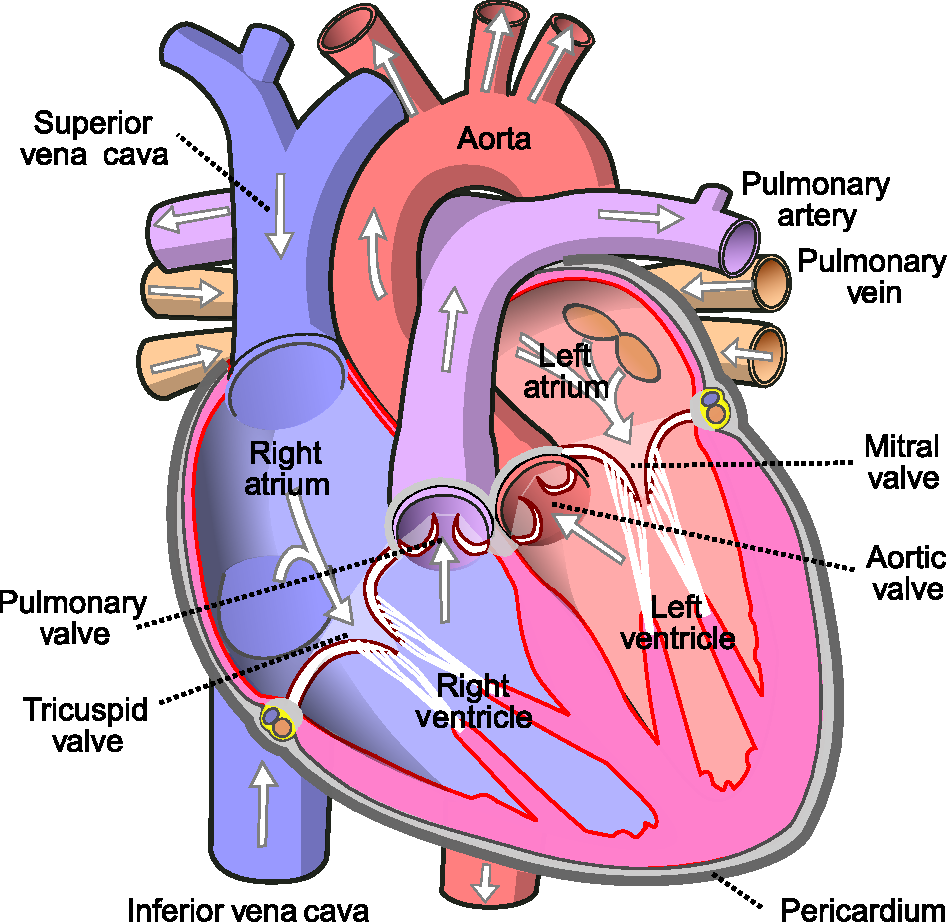
\includegraphics[width=8cm]{figure/Diagram_of_the_human_heart.pdf}
    \caption[Anterior, anatomical view of the structures of a human heart.]{Anterior, anatomical view of a human heart. The primary valves and chambers of the heart are annotated, with arrows indicating the direction of blood flow due to the contractions of the cardiac chambers.
    Image licensed \texttt{CC BY-SA 3.0} from Wikipedia user \href{https://en.wikipedia.org/wiki/User:Wapcaplet}{Wapcaplet}, source: \url{https://en.wikipedia.org/wiki/Heart\#/media/File:Diagram\_of\_the\_human\_heart\_(cropped).svg}
    }
    \label{fig:heart_anatomy}
\end{figure}

A high level overview of the primary valves and chambers within the heart can be found in Figure~\ref{fig:heart_anatomy}.
The upper chambers of the heart, consisting of the right and left atriums, work in cooperation with the lower chambers of the heart, consisting of the left and right ventricles.
The right ventricle pushes blood into the pulmonary artery which connects to the lungs to return oxygenated blood.
The oxygenated blood returns to the heart through the pulmonary veins and enters into the left atrium.
The left atrium collects ad pumps the oxygenated blood into the left ventricle through the mitral valve.
The left ventricle pumps the oxygenated blood out of the heart to the rest of the body through the aorta.
The deoxygenated blood is collected back into the heart through the superior and inferior vena cava and into the right atrium.
The cycle repeats as the right atrium pumps the blood into the right ventricle through the tricuspid valve, allowing the lungs to once again oxygenate the blood.

\begin{figure}[ht]
    \centering
    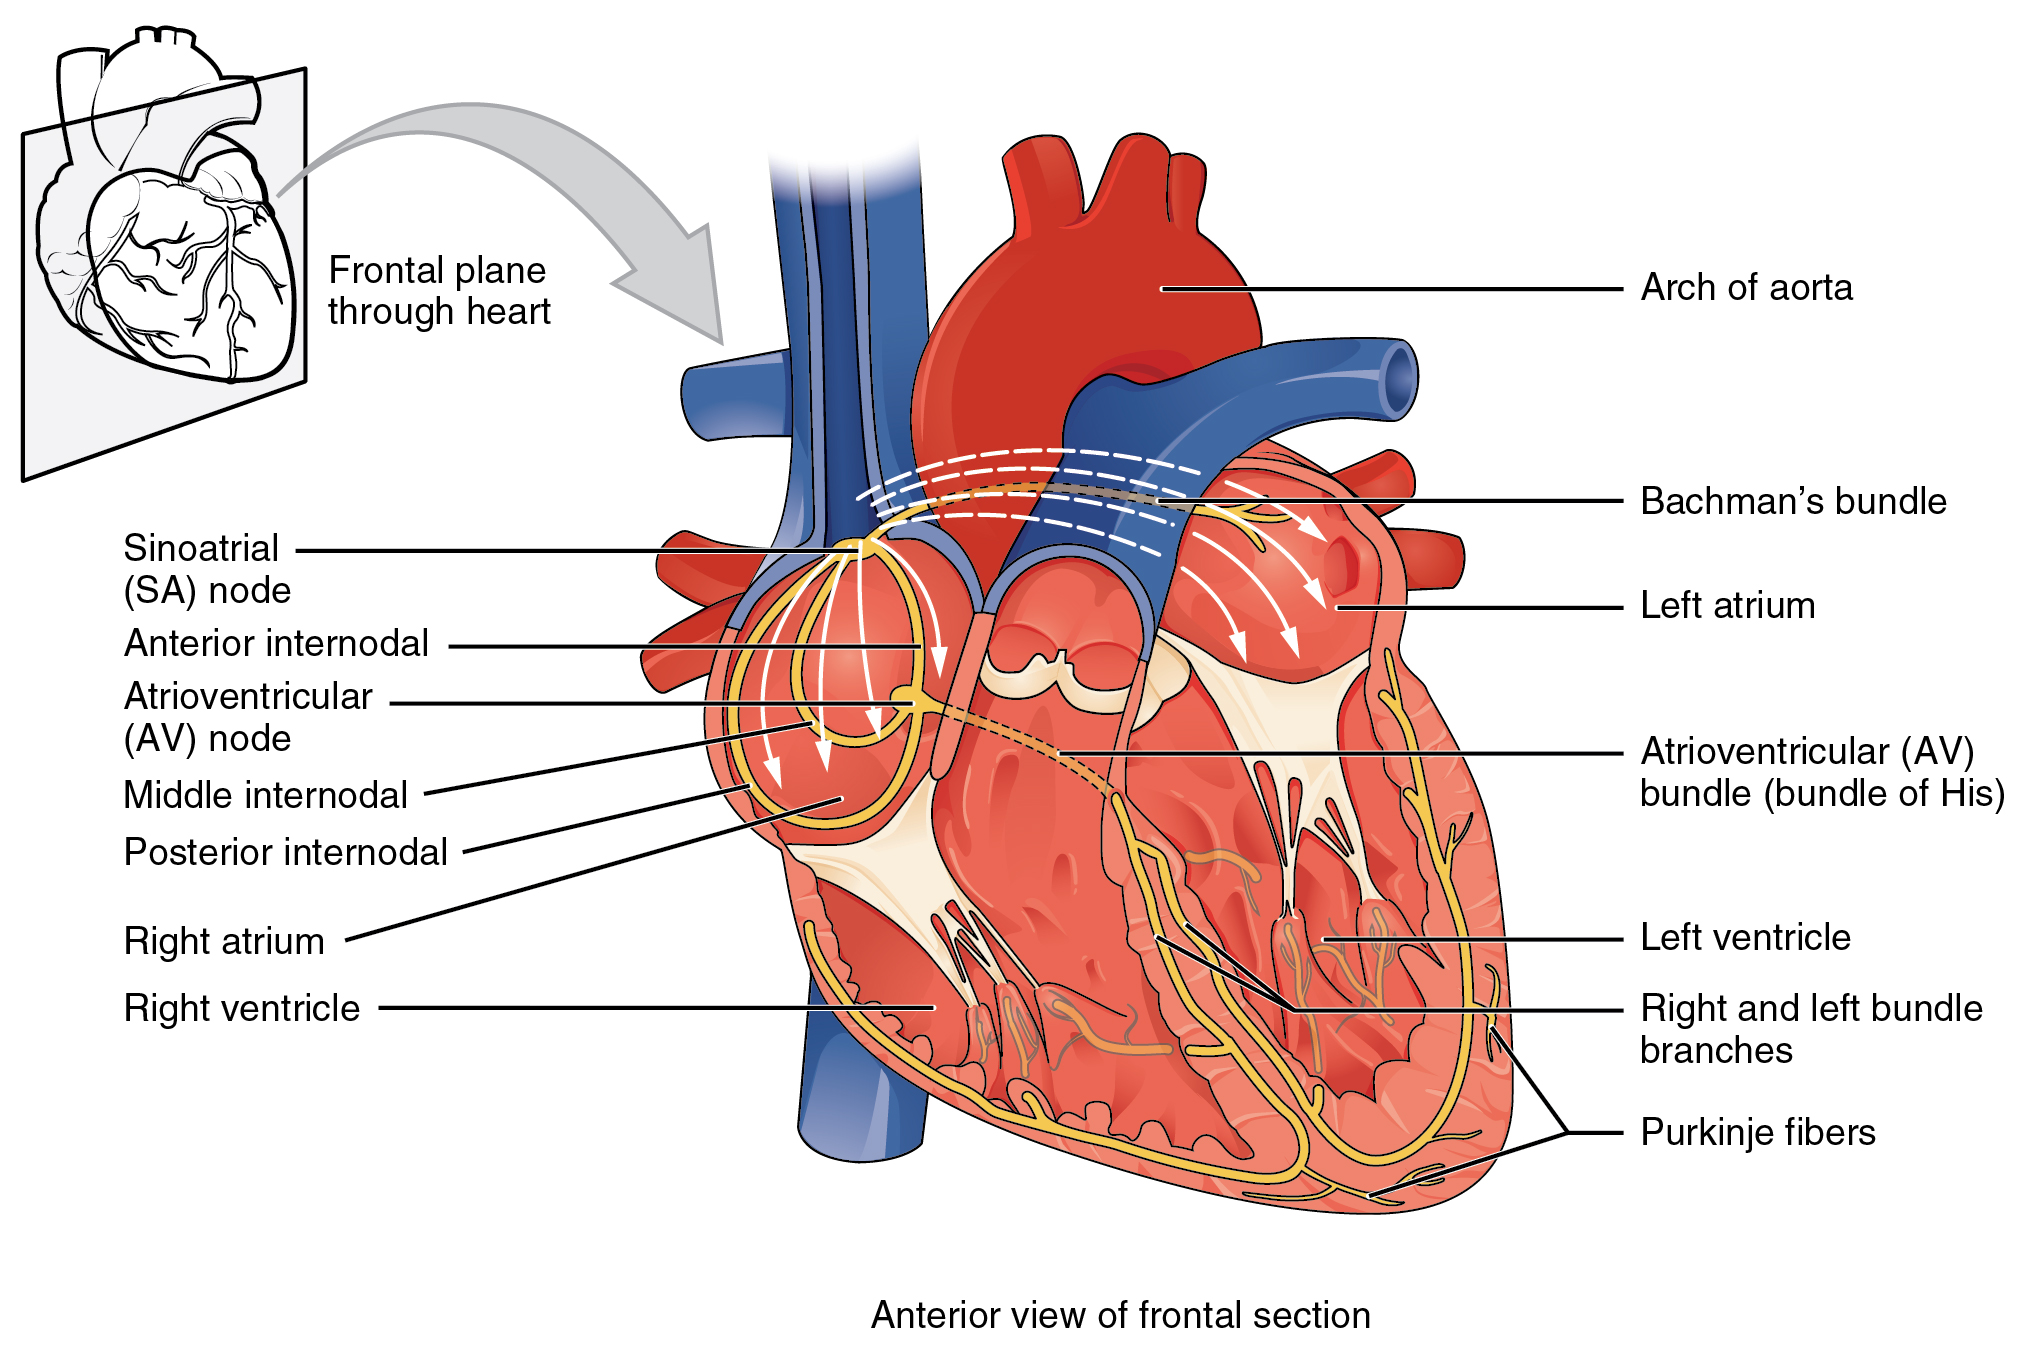
\includegraphics[width=14cm]{figure/conduction-system-of-the-heart.jpeg}
    \caption[Anterior, anatomical view of the conduction system of a human heart.]{Anterior, anatomical view of the conduction system of a human heart. The conducting components of the heart begin with the sinoatrial node and include the internodal pathways, the atrioventricular node, the atrioventricular bundle, the right and left bundle branches, and the Purkinje fibres.
    Image licensed \texttt{CC BY 4.0} from Betts \emph{et al}~\cite{betts-anatomy-and-physiology} on the OpenStax platform, source: \url{https://openstax.org/books/anatomy-and-physiology/pages/19-2-cardiac-muscle-and-electrical-activity\#fig-ch20_02_02}}
    \label{fig:heart_conduction_system}
\end{figure}

Figure~\ref{fig:heart_conduction_system} shows an overview of the primary structures relevant to the cardiac conduction cycle.
Starting at rest, the sinoatrial node initiates an action potential which travels across the right and left atria.
Once the action potential reaches the atrioventricular node, a ~100ms delay occurs to allow the atria to finish pumping blood before the impluse is sent to the atrioventricular bundle.
Once the delay finishes, the impluse sweeps across the atrioventricular bundle, right and left bundle branches, and to the Purkinje fibers.
Ventricular contraction occurs, then the impulse dissipates at the contractile fibers of the ventricle causing the ventricles to repolarize in preparation for the next heartbeat.

\subsection{Electrocardiogram Tracing}

\begin{figure}[ht]
    \centering
    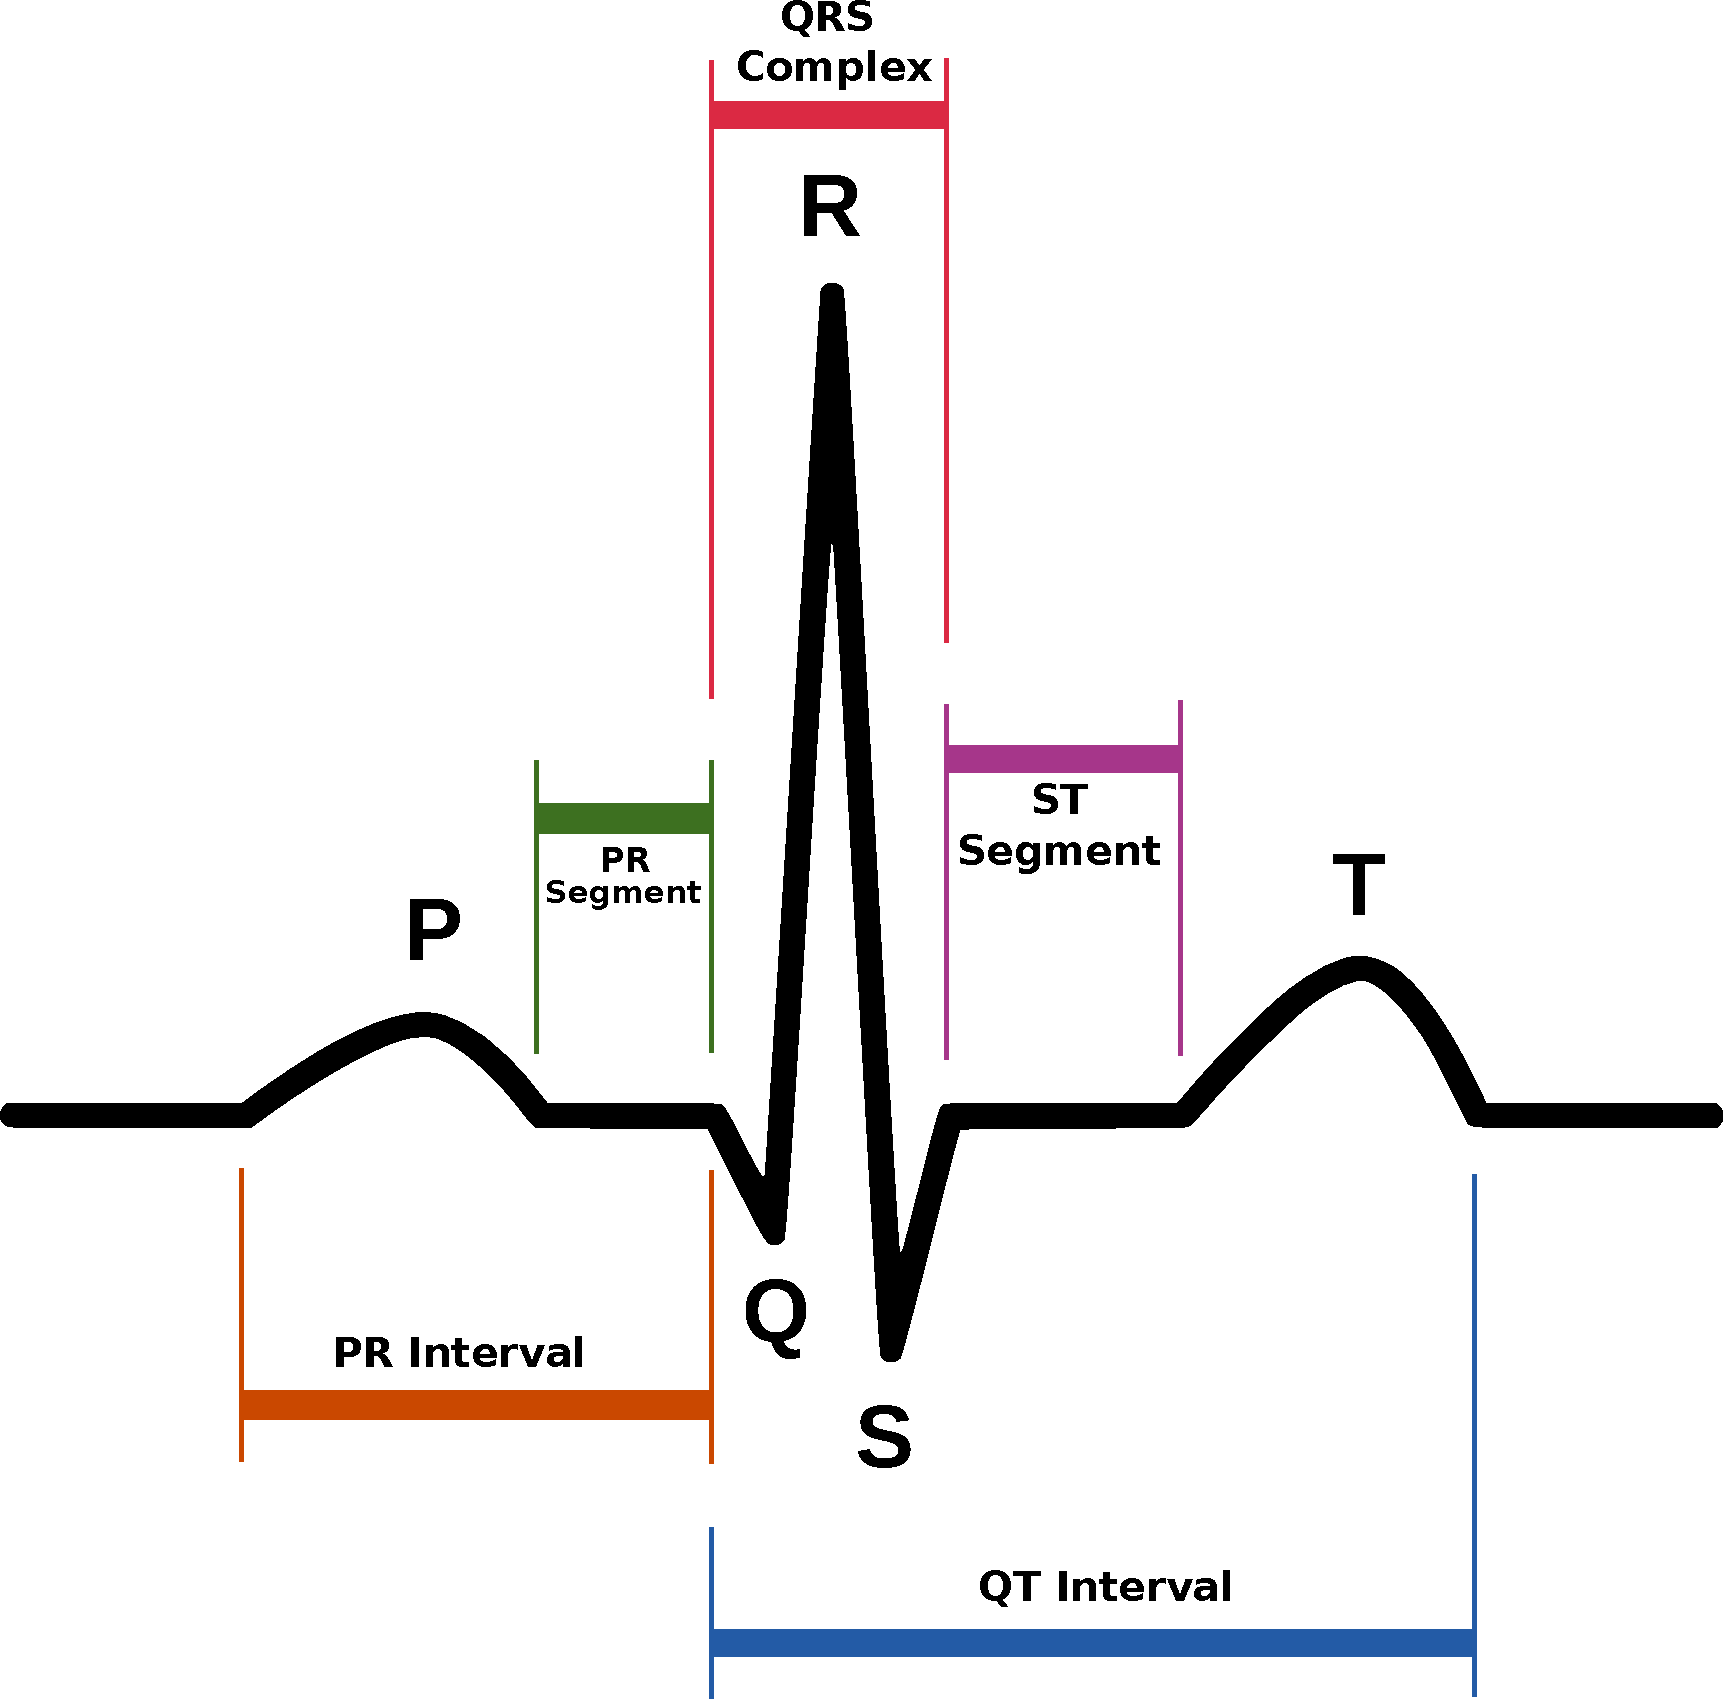
\includegraphics[width=8cm]{figure/PQRST_NormalSinusRhythm.pdf}
    \caption[Normal sinus rhythm \gls{ecg} tracing with PQRST peaks annotated.]{Normal sinus rhythm \gls{ecg} tracing showing the PQRST peaks, the P wave, QRS complex, and T wave along with the PR and QT intervals, plus the PR and ST segments.
    Image belonging to \texttt{public domain} attributed to Anthony Atkielski, source: \url{https://en.wikipedia.org/wiki/Electrocardiography\#/media/File:SinusRhythmLabels.svg}
    }
    \label{fig:pqrst_nsr}
\end{figure}

Within a typical \gls{ecg}, there are five peaks, labeled PQRST respectively, that define the major components of a heartbeat as shown in Figure~\ref{fig:pqrst_nsr}.
The P wave represents the sinoatrial node initiating an impulse action potential and marks the start of a heartbeat.
The PR segment, which starts after the P wave and ends before the QRS complex, represents the delay between the atrial contraction and the propagation of the signal through the atrioventricular bundle.
The QRS complex is the notable large spike in the \gls{ecg}, which represents the electrical impluse traveling through the atrioventricular bundle and bundle branches to the Purkinje fibers.
The ST segment, starting after the QRS complex and ending before the T wave begins, is the phase of the \gls{ecg} where the actual ventricle contraction occurs.
After the ventricle contraction completes, the impulse dissipates and allows the ventricle muscles to relax and repolarize, manifesting as the \gls{ecg} T wave.
A step by step diagram indicating the different \gls{ecg} tracing components and the corresponding cardiac diagram can be found in Figure~\ref{fig:pqrst_heart_conduction_system}

\begin{figure}[hb]
    \centering
    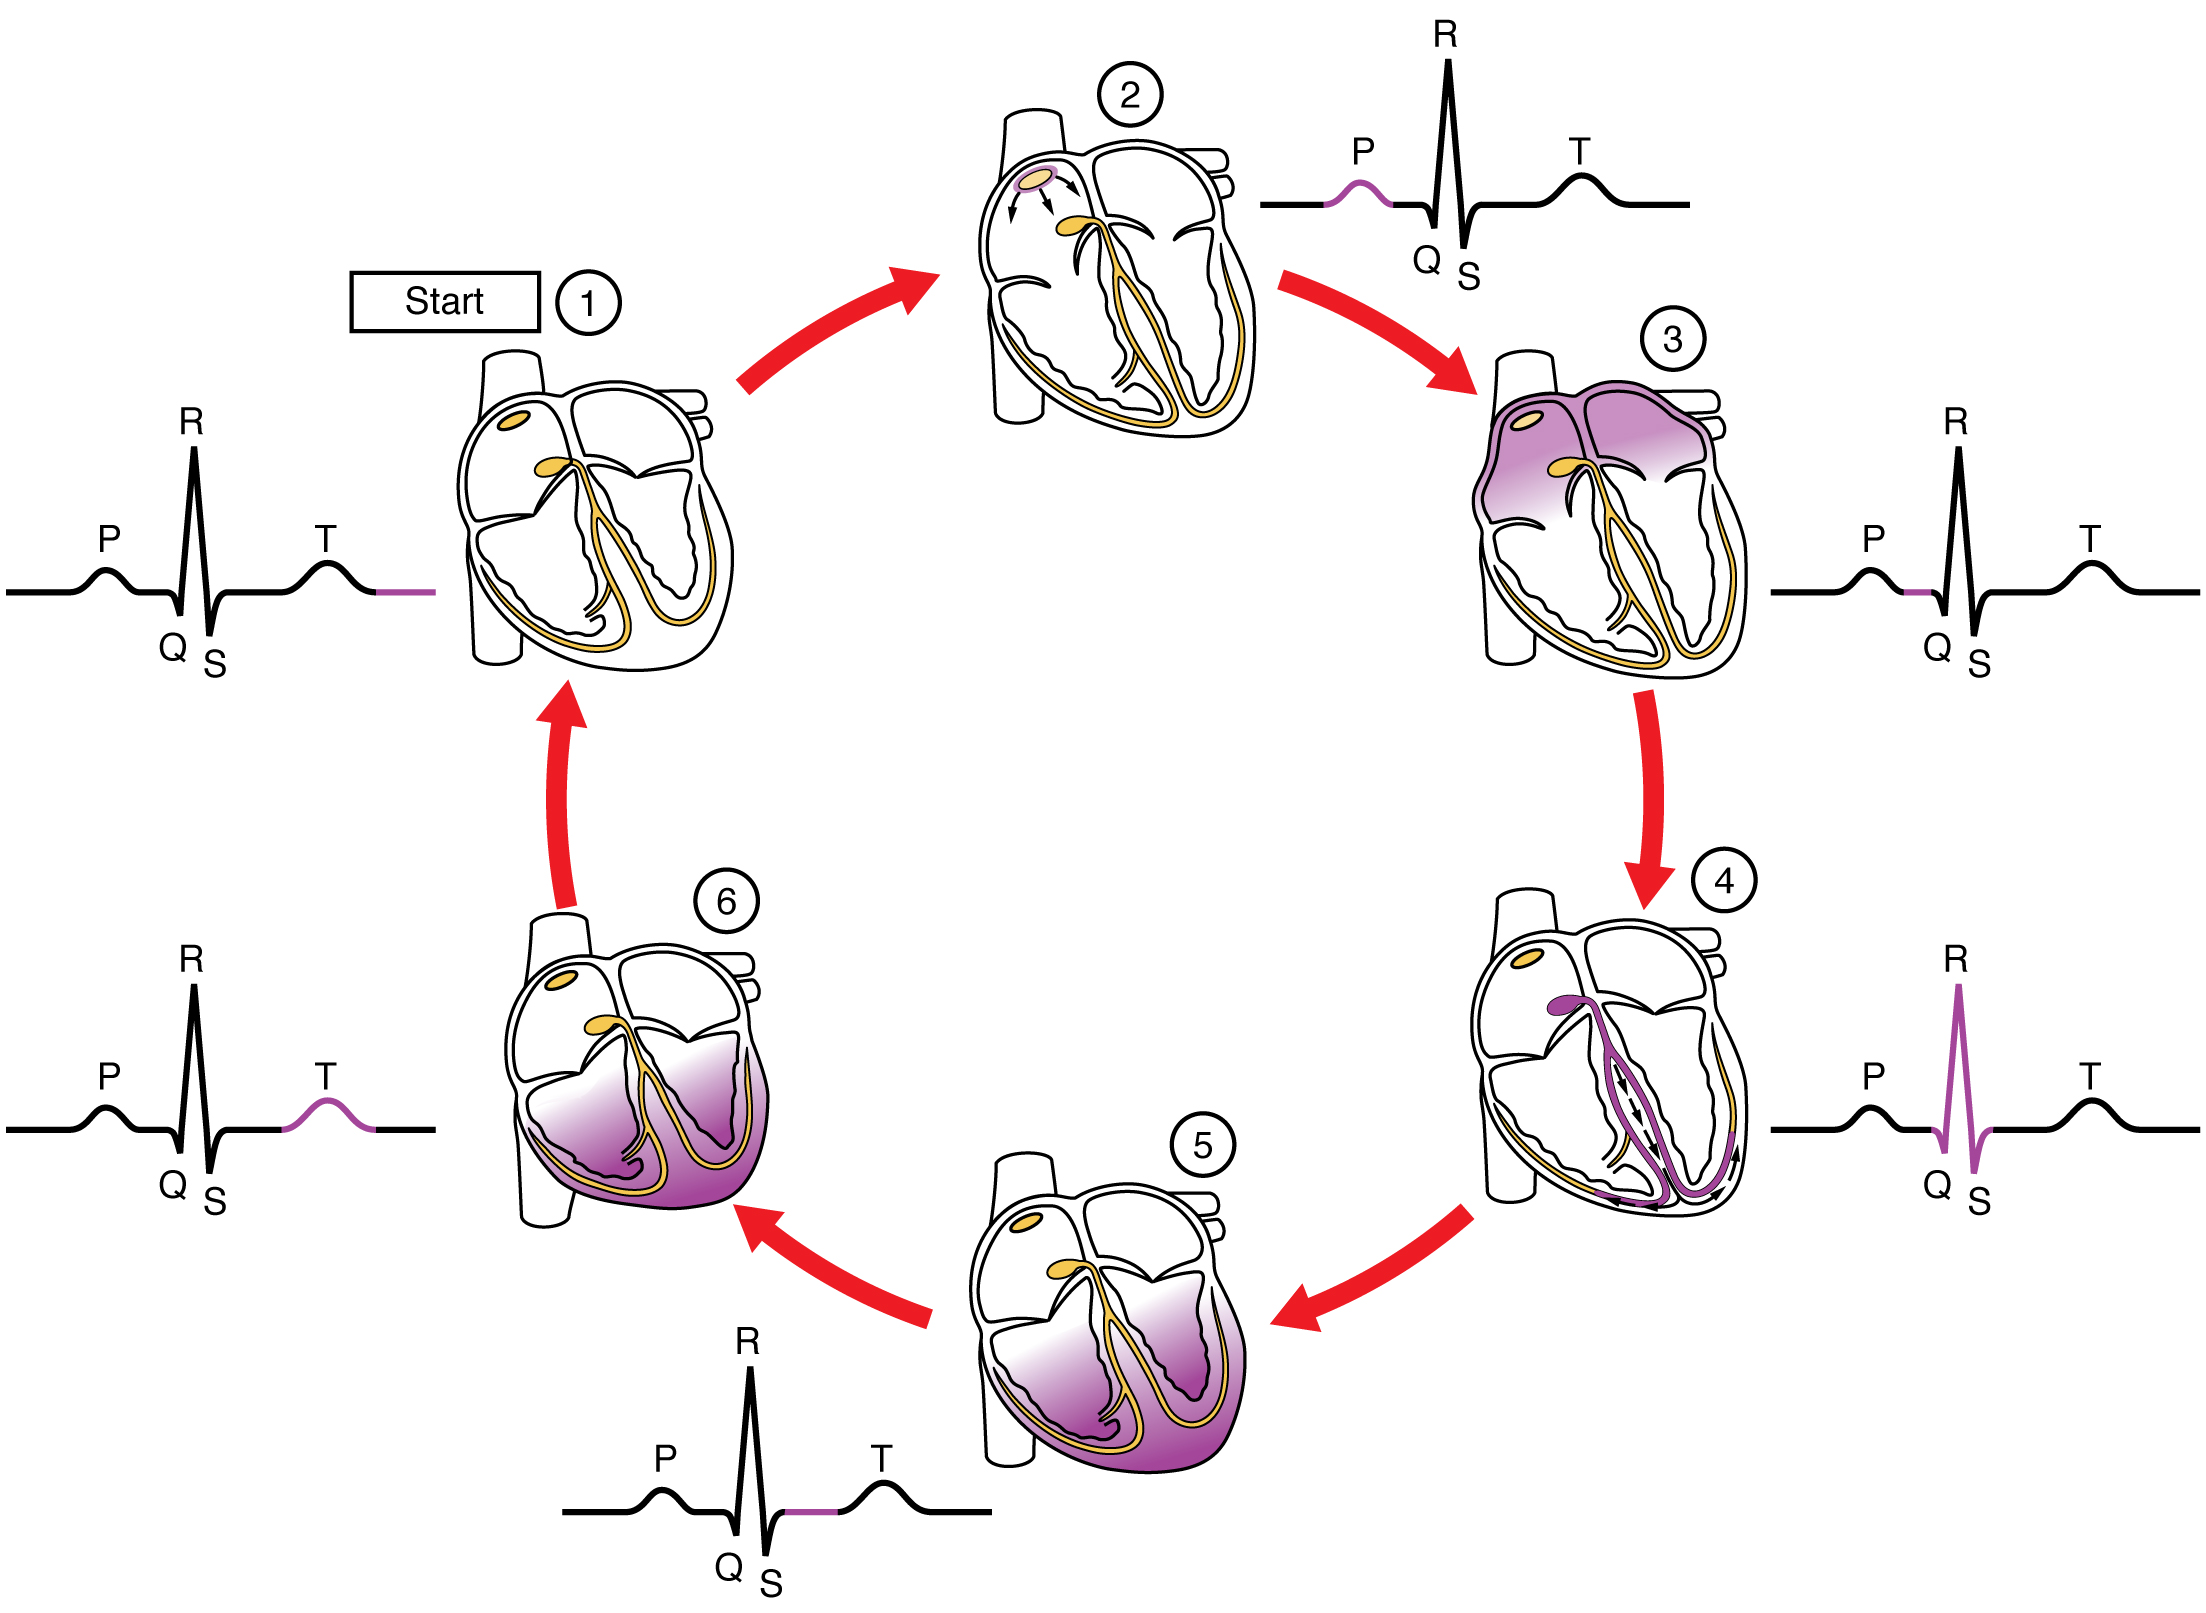
\includegraphics[width=14cm]{figure/pqrst_with_heart_conduction_system.jpeg}
    \caption[Cardiac conduction correlated to ECG tracing waves.]{Cardiac conduction correlated to ECG tracing waves.
    1. The conduction system of the heart is currently at rest, with the ventricles repolarized.
    2. The sinoatrial node begins an action potential which permeates across the atria, causing the \gls{ecg} P wave formation.
    3. A 100ms delay in the impulse occurs which allows the atria to complete pumping blood, showing as the PR segment in the \gls{ecg}.
    4. The impulse proceeds through the atrioventricular bundle and bundle branches to the Purkinje fibers, appearing as the QRS complex in the \gls{ecg}.
    5. The contractile fibers of the ventricles are stimulated by the impulse, causing the ventricles to contract and appears as the ST-segment in the \gls{ecg}.
    6. The impulse dissipates and the ventricular muscles relax, causing the \gls{ecg} T wave formation.
    Image licensed \texttt{CC BY 4.0} from Betts \emph{et al}~\cite{betts-anatomy-and-physiology} on the OpenStax platform, source: \url{https://openstax.org/books/anatomy-and-physiology/pages/19-2-cardiac-muscle-and-electrical-activity\#fig-ch20_02_08}}
    \label{fig:pqrst_heart_conduction_system}
\end{figure}

\section{PhysioNet/CinC 2020 Challenge Overview}

This chapter summarizes the task of multi-label, multi-class classification of \gls{ecg}s as proposed by Perez Alday \emph{et al.}~\cite{physionet_challenge_2020} in the \emph{PhysioNet/CinC 2020 Challenge}.

\subsection{Public Dataset}
The challenge provided a public collection of 43,101 labelled \gls{ecg} records for training.
These public records were sourced from multiple locations, including:

\begin{enumerate}
    \item The China Physiological Signal Challenge (\textbf{CPSC}) 2018~\cite{liu_open_2018} corpus of data, containing 10,330 recordings.
    \item The St. Petersburg Institute of Cardiological Technics (\textbf{INCART}) database of 12-lead arrhythmias~\cite{tihonenko2008st}, containing 74 recordings.
    \item The Physikalisch Technische Bundesanstalt (PTB) contributed datasets \textbf{PTB} Diagnostic \gls{ecg} Database~\cite{NutzungderEKGSignaldatenbankCARDIODATderPTBberdasInternet} and the more recent \textbf{PTB-XL} database~\cite{wagner_ptb-xl_2020}, containing a combined total of 22,353 records
    \item The Georgia 12-lead \gls{ecg} Challenge (\textbf{G12EC}) database, containing 10,344 records.
\end{enumerate}

A separate hold-out set of \gls{ecg} records is sourced from an undisclosed organization containing patients geographically distinct from the publicly available data.
This hold-out set of data is used for the official challenge test phase only and is not available to researchers.
In my analysis, I do not make any distinction between the different \gls{ecg} source locations and combine all of the records into a single repository.
Two \gls{ecg} records (\texttt{Training\_2/Q0400}, \texttt{Training\_2/Q2961} from the CPSC2018 tranche of signals) containing no activity on any leads are excluded from analysis.

\begin{figure}[ht]
    \centering
    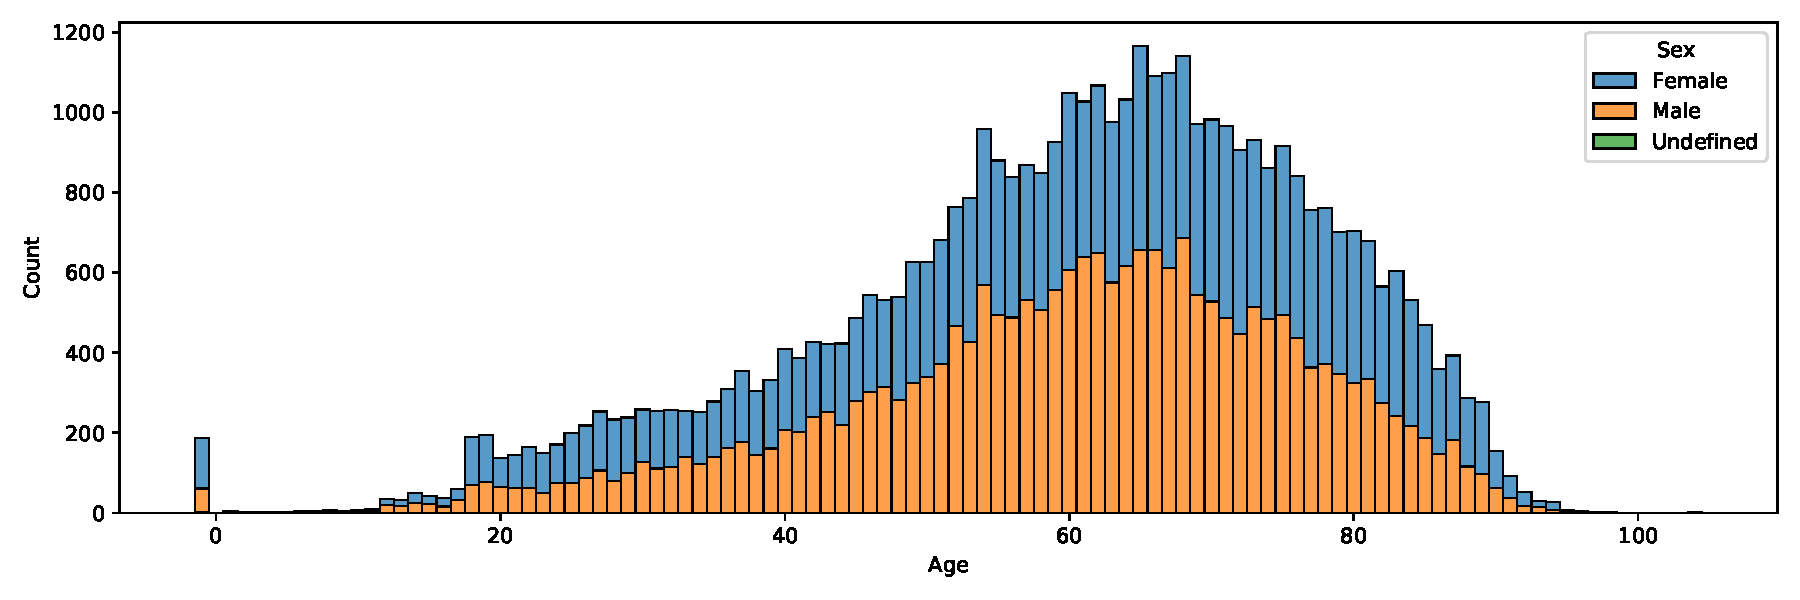
\includegraphics[width=14cm]{figure/age_sex_hist.pdf}
    \caption[Age and sex distribution of the PhysioNet/CinC 2020 public electrocardiogram dataset.]{Age and sex distribution of the PhysioNet/CinC 2020 public electrocardiogram dataset.
    Records with age $<0$ indicate that age is not provided for the given record. The only record that is missing the biological sex metadata is also missing the age metadata.}
    \label{fig:age_sex_hist}
\end{figure}

Each \gls{ecg} record also contains additional metadata in the form of the patient age and biological sex.
There are 187 records that contain an undefined age.
Of the remaining records, the mean patient age is 60.3.
The \gls{ecg} records contained primarily male and female sex, with 46.9\% of the patients in the dataset as female, 53.1\% of the patients as male, and one record that did not have the sex metadata specified.
A histogram showcasing the distribution of the age and sex in our dataset can be found in Figure~\ref{fig:age_sex_hist}.

\subsection{Diagnosed Labels}

\begin{table}[t]
    \caption{\label{tab:labels_snomed_ct} Evaluated SNOMED CT codes with definition, count and percentage in dataset.}
    \vspace{2 mm}
    \centerline{\begin{tabular}{@{}ll@{}l@{}r@{}}
    SNOMED & Abbr. & Diagnosis & Count (\%) \\ \hline
    270492004 & IAVB & 1st degree av block & 2394 (5.6\%) \\
    164889003 & AF & atrial fibrillation & 3475 (8.0\%) \\
    164890007 & AFL & atrial flutter & 314 (0.7\%) \\
    426627000 & Brady & bradycardia & 288 (0.7\%) \\
    713427006 & CRBBB & complete right bundle branch block & 683 (1.6\%) \\
    713426002 & IRBBB & incomplete right bundle branch block & 1611 (3.7\%) \\
    445118002 & LAnFB & left anterior fascicular block & 1806 (4.2\%) \\
    39732003 & LAD & left axis deviation & 6086 (14.1\%)  \\
    164909002 & LBBB & left bundle branch block & 1041 (2.4\%) \\
    251146004 & LQRSV & low QRS voltages & 556 (1.3\%) \\
    698252002 & {{NSIVCB }} & nonspecific intraventricular conduction & 997 (2.3\%) \\
    10370003 & PR & pacing rhythm & 299 (0.7\%) \\
    284470004 & PAC & premature atrial contraction & 1729 (4.0\%) \\
    427172004 & PVC & premature ventricular contractions & 188 (0.4\%) \\
    164947007 & LPR & prolonged PR interval & 340 (0.7\%) \\
    111975006 & LQT & prolonged QT interval & 1513 (3.5\%) \\
    164917005 & QAb & Q wave abnormal & 1013 (2.4\%) \\
    47665007 & RAD & right axis deviation & 427 (1.0\%) \\
    59118001 & RBBB & right bundle branch block & 2402 (5.6\%) \\
    427393009 & SA & sinus arrhythmia & 1240 (2.9\%) \\
    426177001 & SB & sinus bradycardia & 2359 (5.5\%) \\
    426783006 & SNR & sinus rhythm & 20846 (48.4\%)  \\
    427084000 & STach & sinus tachycardia & 2402 (5.6\%) \\
    63593006 & SVPB & supraventricular premature beats & 215 (0.5\%) \\
    164934002 & TAb & T wave abnormal & 4673 (10.8\%)  \\
    59931005 & TInv & T wave inversion & 1112 (2.6\%) \\
    17338001 & VPB & ventricular premature beats & 365 (0.8\%) \\ \hline
    \end{tabular}}
\end{table}

Each record in our available dataset is labelled with at least one numerical \gls{snomed} clinical term (CT).
For the purpose of the challenge, a subset of 27 codes/labels have been selected for classification.
All other codes are ignored in this study.
Please refer to Table~\ref{tab:labels_snomed_ct} for the labels, abbreviations, counts, and proportion within the dataset.

\begin{description}
    \item[\gls{iavb}] This is when there is an abnormally long delay between the electrical impulse from the atria, through the ventricular node, to the ventricles. On the \gls{ecg}, this is detected by the presence of a PR interval longer than 200ms~\cite{carroz_pseudo-pacemaker_2010}.
    \item[\gls{af}]
    \item[\gls{afl}]
    \item[\gls{brady}]
    \item[\gls{crbbb}]
    \item[\gls{irbbb}]
    \item[\gls{lanfb}]
    \item[\gls{lad}]
    \item[\gls{lbbb}]
    \item[\gls{lqrsv}]
    \item[\gls{nsivcb}]
    \item[\gls{pr}]
    \item[\gls{pac}]
    \item[\gls{pvc}]
    \item[\gls{lpr}]
    \item[\gls{lqt}]
    \item[\gls{qab}]
    \item[\gls{rad}]
    \item[\gls{rbbb}]
    \item[\gls{sa}]
    \item[\gls{sb}]
    \item[\gls{snr}]
    \item[\gls{stach}]
    \item[\gls{svpb}]
    \item[\gls{tab}]
    \item[\gls{tinv}]
    \item[\gls{vpb}]
\end{description}

\subsection{Scoring Function}

% We plot an equation in figure \ref{fig:plot}.

% \begin{figure}
%     \centering
%     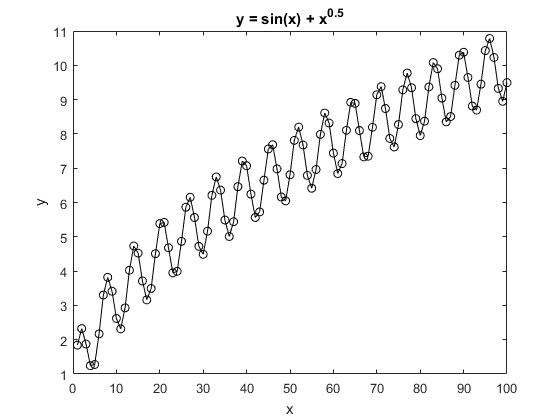
\includegraphics[keepaspectratio=true, width=0.9\textwidth]{\main/figure/plot}
%     \caption[A supporting figure] {A graph of $y = \sin(x) + \sqrt{x}$}
%     \label{fig:plot}
%     % Put the label *after* the caption, but inside the float
% \end{figure}

\end{document}